\documentclass[notes,blackandwhite,mathsans,usenames,dvipsnames]{beamer}

\usepackage{amsmath}
\usepackage{amssymb}
\usepackage{graphicx}
\usepackage{fancybox}
\usepackage{booktabs}
\usepackage{multirow,pxfonts}
\usepackage{cmbright}
\usepackage{xcolor}
\usepackage{color}
\usepackage{enumitem}
\usepackage{animate}
\usepackage{changepage}

\usepackage[T1]{fontenc}
\fontencoding{T1}  
\usepackage[utf8]{inputenc}


\usefonttheme{default}
\setbeamercovered{invisible}
\beamertemplatenavigationsymbolsempty

\makeatletter
\setbeamertemplate{footline}
{
  \leavevmode
  \hbox{
  \begin{beamercolorbox}[wd=0.97\paperwidth,ht=2.25ex,dp=2ex,right]{}
{\color{mcxs2} \insertframenumber{} / \inserttotalframenumber}
  \end{beamercolorbox}}%
}




\definecolor{mcxs1}{HTML}{05386B}
\definecolor{mcxs2}{HTML}{379683}
\definecolor{mcxs3}{HTML}{5CDB95}
\definecolor{mcxs4}{HTML}{8EE4AF}
\definecolor{mcxs5}{HTML}{EDF5E1}
\setbeamercolor{frametitle}{fg=mcxs2}
\AtBeginDocument{\color{mcxs1}}

\setbeamercolor{itemize item}{fg=mcxs1}
\setbeamercolor{itemize subitem}{fg=mcxs2}
\setbeamercolor{enumerate item}{fg=mcxs1}
\setbeamercolor{description item}{fg=mcxs1}

\setbeamertemplate{itemize item}[triangle]
\setbeamertemplate{itemize subitem}[circle]



\begin{document}
%\fontfamily{pag}\selectfont
%\setbeamerfont{title}{family=\fontfamily{pag}\selectfont}
%\setbeamerfont{frametitle}{family=\fontfamily{pag}\selectfont}
%\setbeamerfont{framesubtitle}{family=\fontfamily{pag}\selectfont}






{\setbeamercolor{background canvas}{bg=mcxs4}
\begin{frame}

\vspace{1cm}
\begin{tabular}{rl}
&\textbf{\LARGE\color{purple} Macroeconometrics}\\[8ex]
\textbf{\Large Lecture 12}&\textbf{\Large\color{mcxs2}SVAR Tools}\\[19ex]
&\textbf{Tomasz Wo\'zniak}\\[1ex]
&{\small\color{mcxs2} Department of Economics}\\
&{\small\color{mcxs2}University of Melbourne}
\end{tabular}

\end{frame}
}






{\setbeamercolor{background canvas}{bg=mcxs4}
\begin{frame}

\vspace{1cm}\textbf{\color{mcxs2}SVAR Model of the Australian Economy}

\bigskip\textbf{\color{purple}Impulse response functions}

\bigskip\textbf{\color{mcxs2}Forecast error variance decomposition}

%\bigskip\textbf{\color{mcxs2}Historical decomposition}


\small
\vspace{1cm} Compulsory readings: \scriptsize

\smallskip{\color{mcxs2}Kilian \& L\"utkepohl (2017) Chapter 4: Structural VARs Tools, Structural Vector Autoregressive Analysis}


\small
\bigskip Useful readings: \scriptsize

\smallskip{\color{mcxs2}Dungey \& Pagan (2009) Extending a SVAR Model of the Australian Economy, Economic Record}


\small
\bigskip Materials: \scriptsize

\smallskip{\color{mcxs2}R file} \texttt{L12 mcxs.R} {\color{mcxs2}and data file} \texttt{AU-SVAR-data.zip} {\color{mcxs2}for the reproduction of the results}


\end{frame}
}







{\setbeamercolor{background canvas}{bg=mcxs4}
\begin{frame}

\bigskip\textbf{\color{mcxs1}Objectives.}
\begin{itemize}[label=$\blacktriangleright$]
\item {\color{mcxs1}To present the impulse response functions as the dynamic causal effects}
\item {\color{mcxs1}To analyse shocks' contributions to business cycle and inflation}
\item {\color{mcxs1}To introduce a benchmark model of the Australian economy}
\end{itemize}

\bigskip\textbf{\color{mcxs2}Learning outcomes.}
\begin{itemize}[label=$\blacktriangleright$]
\item {\color{mcxs2}Understanding when a structural shock is an important driver of business cycles}
\item {\color{mcxs2}Visualising of economically interpretable effects}
\item {\color{mcxs2}Interpreting IRFs and FEVDs}
\end{itemize}

\end{frame}
}









{\setbeamercolor{background canvas}{bg=mcxs4}
\begin{frame}

\begin{adjustwidth}{-0.5cm}{0cm}
\Large
\textbf{{\color{mcxs1}SVAR Model of the} {\color{mcxs2}Australian Economy}}\\[31ex]
\small{\color{mcxs1}Inspired by Dungey \& Pagan (2009)}
\end{adjustwidth}

\end{frame}
}





\begin{frame}{SVAR Model of the Australian Economy}

\begin{align*}
y_t &= \mu_0 + A_1y_{t-1}+ \dots + A_py_{t-p} + Bu_t\\
u_t|Y_{t-1} &\sim iid(\mathbf{0}_N,I_N)
\end{align*}


\bigskip\textbf{SVAR for a small-open economy}
\begin{itemize}[label=\textbullet,leftmargin = *]
\item {\color{mcxs2}Distinguishes foreign and domestic variables}
\item {\color{mcxs2}The} {\color{purple}small-open economy} {\color{mcxs2}assumption:}
	\begin{itemize}[label=\textbullet,leftmargin = 0.5cm]
	\item {\color{mcxs2}Australia receives foreign shocks}
	\item {\color{mcxs2}foreign sector is not affected by Australian domestic shocks}
	\end{itemize}
\item {\color{mcxs2}Identification of foreign shocks}
\item {\color{mcxs2}Identification of domestic shocks}
\end{itemize}

\end{frame}




\begin{frame}{SVAR Model of the Australian Economy}
\footnotesize
\begin{align*}
\begin{bmatrix} {\color{mcxs1}y_t^{f}} \\ {\color{purple}y_t^d} \end{bmatrix} &= \begin{bmatrix} {\color{mcxs1}\mu_{0.1}}\\{\color{purple}\mu_{0.2}} \end{bmatrix}  + \begin{bmatrix} {\color{mcxs1}A_{1.11}} & {\color{purple}\mathbf{0}_{6\times6}} \\ A_{1.21} & {\color{purple}A_{1.22}} \end{bmatrix} \begin{bmatrix} {\color{mcxs1}y_{t-1}^{f}} \\ {\color{purple}y_{t-1}^d} \end{bmatrix} + \dots + \begin{bmatrix} {\color{mcxs1}B_{11}} & {\color{purple}\mathbf{0}_{6\times6}} \\ B_{21} & {\color{purple}B_{22}} \end{bmatrix} \begin{bmatrix} {\color{mcxs1}u_t^{f}} \\ {\color{purple}u_t^d} \end{bmatrix} \\[2ex]
{\color{mcxs1}y_t^{f\prime}} &= \begin{bmatrix} {\color{mcxs1}rgdp_t} & {\color{mcxs1}cpi_t} & {\color{mcxs1}FFR_t} & {\color{mcxs1}sp500_t} & {\color{mcxs1}tot_t} & {\color{mcxs1}rex_t} \end{bmatrix}\\
{\color{purple}y_t^{d\prime}} &= \begin{bmatrix} {\color{purple}rgne_t} & {\color{purple}rgdp_t} & {\color{purple}cpi_t} & {\color{purple}CR_t} & {\color{purple}rtwi_t} & {\color{purple}aord_t} \end{bmatrix}\\
{\color{mcxs1}u_t^{f\prime}} &= \begin{bmatrix} {\color{mcxs1}u_{1.t}} & {\color{mcxs1}u_{2.t}} & {\color{mcxs1}u_{3.t}^{us.mps}} & {\color{mcxs1}u_{4.t}} & {\color{mcxs1}u_{5.t}} & {\color{mcxs1}u_{6.t}} \end{bmatrix}\\
{\color{purple}u_t^{d\prime}} &= \begin{bmatrix} {\color{purple}u_{7.t}} & {\color{purple}u_{8.t}} & {\color{purple}u_{9.t}} & {\color{purple}u_{10.t}^{au.mps}} & {\color{purple}u_{11.t}} & {\color{purple}u_{12.t}} \end{bmatrix}
\end{align*}

\bigskip\textbf{Foreign block.}\\ \scriptsize
${\color{mcxs1}rgdp_t}$ {\color{mcxs2}-- real GDP,}
${\color{mcxs1}cpi_t}$ {\color{mcxs2}-- CPI,}
${\color{mcxs1}FFR_t}$ {\color{mcxs2}-- federal funds rate,}
${\color{mcxs1}sp500_t}$ {\color{mcxs2}-- S\&P 500 index,}
${\color{mcxs1}tot_t}$ {\color{mcxs2}-- Australian terms of trade,}
${\color{mcxs1}rex_t}$ {\color{mcxs2}-- Australian real export}

\footnotesize\bigskip\textbf{Australian block.}\\ \scriptsize
${\color{purple}rgne_t}$ {\color{mcxs2}-- real gross national expenditure,}
${\color{purple}rgdp_t}$ {\color{mcxs2}-- real GDP,}
${\color{purple}cpi_t}$ {\color{mcxs2}-- CPI,}\\
${\color{purple}CR_t}$ {\color{mcxs2}-- cash rate,}
${\color{purple}rtwi_t}$ {\color{mcxs2}-- real trade weighted index,}
${\color{purple}aord_t}$ {\color{mcxs2}-- All Ordinaries Index}

\footnotesize\bigskip\textbf{Shocks of interest.}\\ \scriptsize
${\color{purple}u_{10.t}^{au.mps}}$ {\color{mcxs2}-- Australian monetary policy shock}\\[1ex]
${\color{mcxs1}u_{3.t}^{us.mps}}$ {\color{mcxs2}-- US  monetary policy shock}
\end{frame}



\begin{frame}{SVAR Model of the Australian Economy}

$$
\begin{bmatrix} {\color{mcxs1}y_t^{f}} \\ {\color{purple}y_t^d} \end{bmatrix} = \begin{bmatrix} {\color{mcxs1}\mu_{0.1}}\\{\color{purple}\mu_{0.2}} \end{bmatrix}  + \begin{bmatrix} {\color{mcxs1}A_{1.11}} & {\color{purple}\mathbf{0}_{6\times6}} \\ A_{1.21} & {\color{purple}A_{1.22}} \end{bmatrix} \begin{bmatrix} {\color{mcxs1}y_{t-1}^{f}} \\ {\color{purple}y_{t-1}^d} \end{bmatrix} + \dots + \begin{bmatrix} {\color{mcxs1}B_{11}} & {\color{purple}\mathbf{0}_{6\times6}} \\ B_{21} & {\color{purple}B_{22}} \end{bmatrix} \begin{bmatrix} {\color{mcxs1}u_t^{f}} \\ {\color{purple}u_t^d} \end{bmatrix}
$$


\bigskip\textbf{SVAR for a small-open economy}
\begin{description}
\item[${\color{mcxs1}B_{11}}$] {\color{mcxs2}-- identification of foreign shocks: lower-triangular matrix}
\item[${\color{purple}B_{22}}$] {\color{mcxs2}-- identification of domestic shocks: lower-triangular matrix}
\item[${\color{purple}B_{12}}={\color{purple}\mathbf{0}_{6\times6}}$] {\color{mcxs2}-- small-open economy assumption}
\item[${\color{purple}A_{l.12}}={\color{purple}\mathbf{0}_{6\times6}}$] {\color{mcxs2}-- small-open economy assumption (not imposed)}
\item[$B_{21}$] {\color{mcxs2}-- small-open economy assumption: foreign shocks affect domestic variables}
\end{description}

\end{frame}


{\setbeamercolor{background canvas}{bg=mcxs4}
\begin{frame}{SVAR Model of the Australian Economy}
\centering
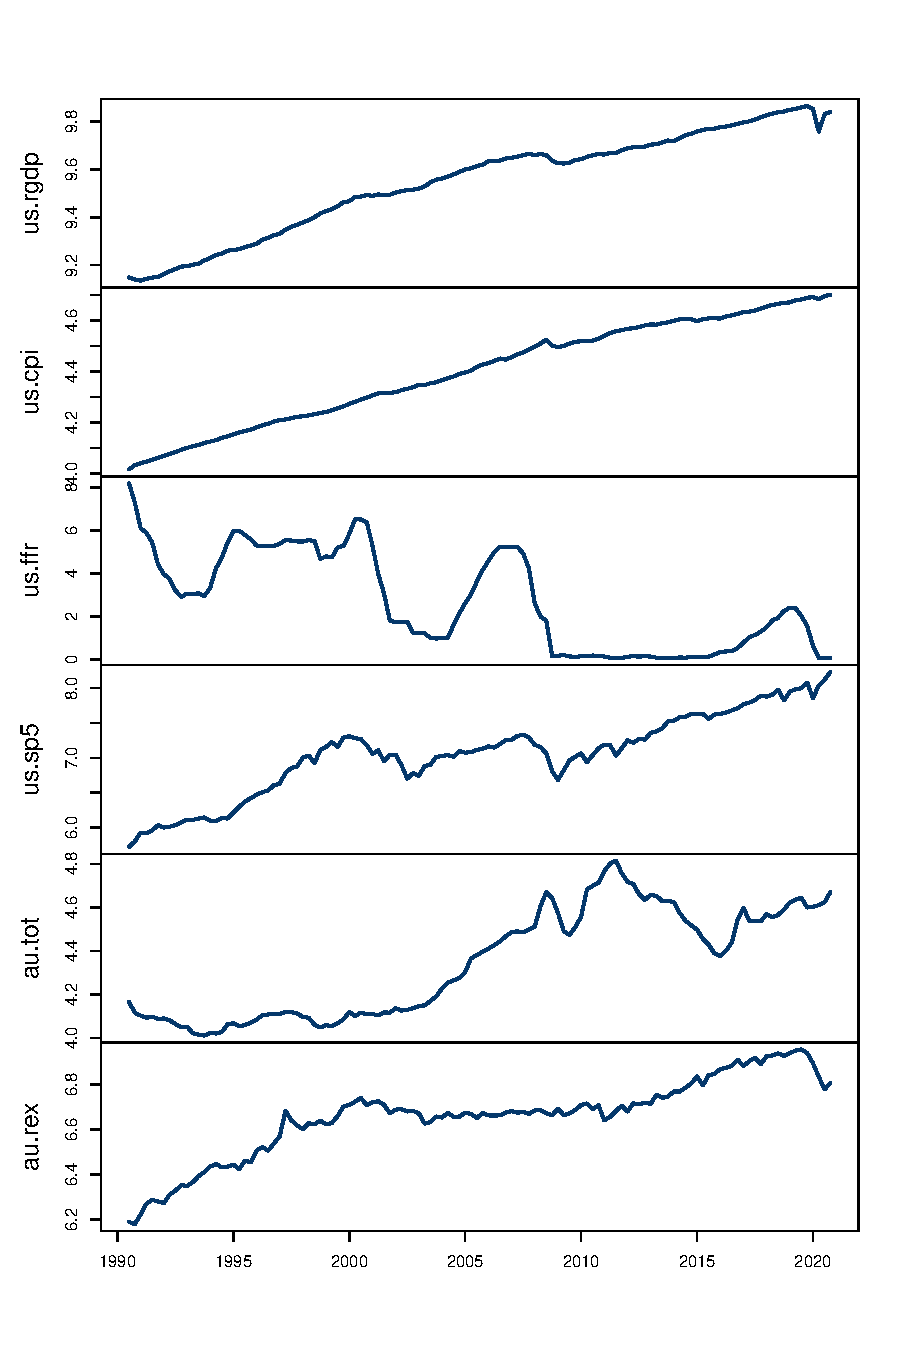
\includegraphics[scale=0.37, trim=1.5cm 0cm 0cm 0cm]{data-foreign.pdf}
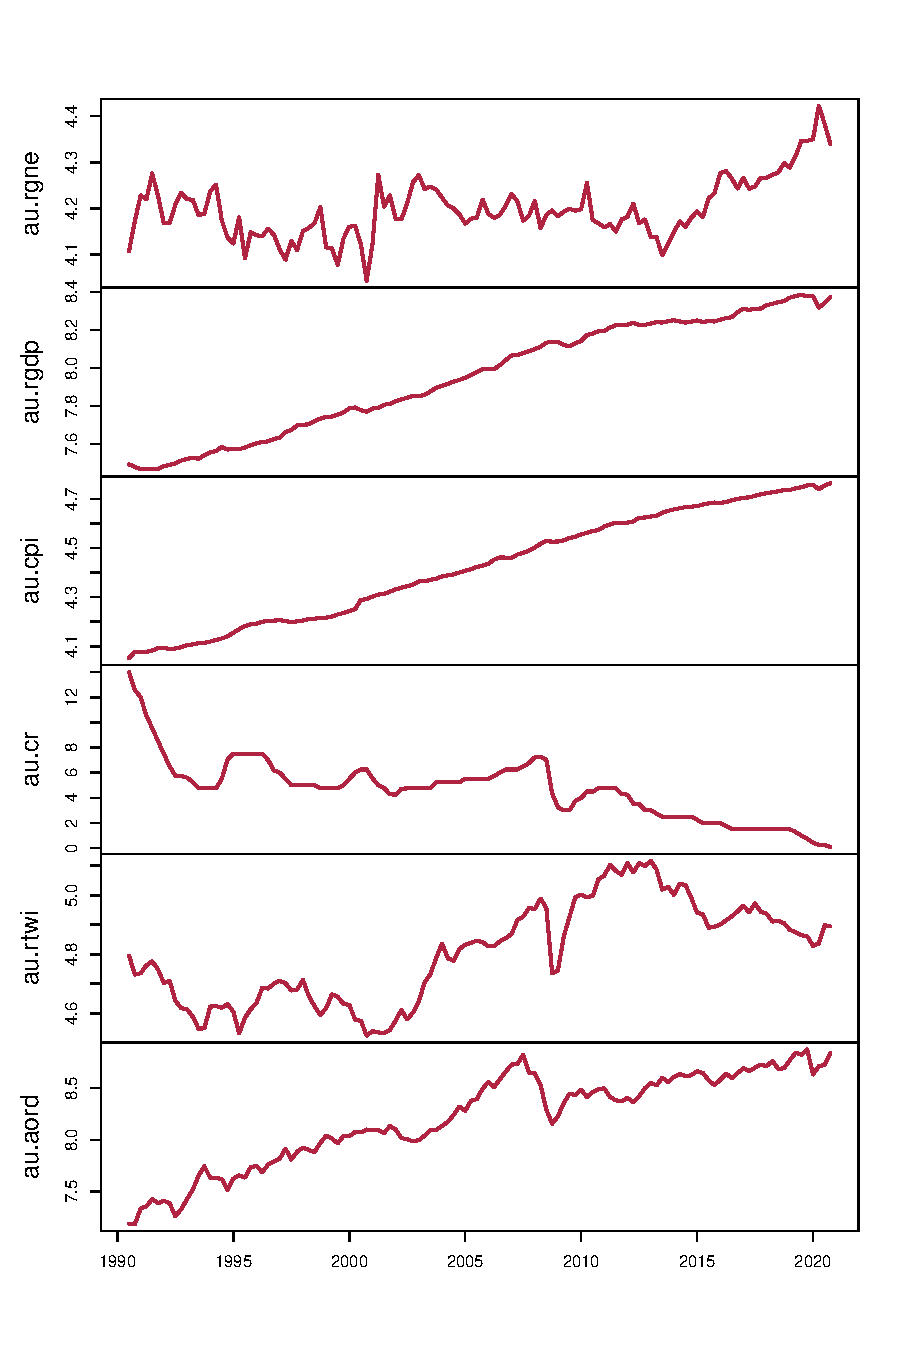
\includegraphics[scale=0.37, trim=0.6cm 0cm 1cm 0cm]{data-domestic.pdf}

\end{frame}
}




\begin{frame}{SVAR Model of the Australian Economy}

\textbf{Minnesota prior}

{\color{mcxs2}All of the results are reported for} $\kappa_1\in\left\{0.02^2,1\right\}$ {\color{mcxs2}and}
$$ \underline{A} = \begin{bmatrix} \mathbf{0}_{1\times N} \\ {\color{purple}\kappa_3}I_N \\ \mathbf{0}_{N(p-1)\times N} \end{bmatrix} $$
{\color{mcxs2}with} ${\color{purple}\kappa_3}=1$, $p=4$, {\color{mcxs2}and} $S=50,000$.

\bigskip {\color{mcxs2}The results are heavily dependent on prior hyper-parameters.}

\end{frame}







{\setbeamercolor{background canvas}{bg=mcxs4}
\begin{frame}

\begin{adjustwidth}{-0.5cm}{0cm}
\vspace{8.3cm}\Large
\textbf{{\color{mcxs1}Impulse response} {\color{mcxs2}functions}}
\end{adjustwidth}

\end{frame}
}





\begin{frame}{Impulse response functions}

\bigskip\textbf{Definition.}

Impulse response functions {\color{mcxs2}to orthogonal shocks computed for an empirically relevant SVAR model are considered the dynamic causal effects of the underlying shocks} $u_t$ {\color{mcxs2}on economic measurements} $y_t$.


\begin{align*}
\frac{\partial y_{n.t+i}}{\partial u_{j.t}}&=\theta_{nj.i}\\
\frac{\partial y_{t+i}}{\partial u_t}&=\underset{N\times N}{\Theta_i}
\end{align*}

\begin{description}
\item[$\theta_{nj.i}$] {\color{mcxs2}-- response of $n$th variable to $j$th shock $i$ periods after shock's occurrence}
\item[$\Theta_i$] {\color{mcxs2}-- responses of all of the variables to all of the shocks $i$ periods after shock's occurrence}
\end{description}
{\color{mcxs2}for $i=0,1,\dots,h$ and $n,j=1,\dots,N$}

\end{frame}




\begin{frame}{Impulse response functions}

\bigskip\textbf{VAR(1) representation of RF VAR(p) model.}
\begin{align*}
Y_t &= \mathbf{A}Y_{t-1} + E_t\\
&= E_t + \mathbf{A}E_{t-1} + \mathbf{A}^2E_{t-2} + \dots\\[2ex]
y_t &= JY_t\\
&= JE_t + J\mathbf{A}J'JE_{t-1} + J\mathbf{A}^2J'JE_{t-2} + \dots\\
&= \epsilon_t + J\mathbf{A}J'\epsilon_{t-1} + J\mathbf{A}^2J'\epsilon_{t-2} + \dots\\
&= \Phi_0\epsilon_t + \Phi_1\epsilon_{t-1} + \Phi_2\epsilon_{t-2} + \dots\\[2ex]
\frac{\partial y_{t+i}}{\partial \epsilon_t} &= J\mathbf{A}^iJ' = \Phi_j
\end{align*}

{\color{mcxs2}Matrices} $\Phi_i$ {\color{purple}do not identify the effects of interest} {\color{mcxs2}because they represent responses to correlated shocks.}

\bigskip\tiny$$
\mathbf{A} = \begin{bmatrix}A_1 & A_2 &\dots& A_p\\ &I_{N(p-1)}&&\mathbf{0}_{N(p-1)\times N} \end{bmatrix}\quad
E_t' = \begin{bmatrix}\epsilon_t' & \mathbf{0}_{1\times N(p-1)} \end{bmatrix}\quad
J = \begin{bmatrix} I_{N} & \mathbf{0}_{N\times N(p-1)} \end{bmatrix}
$$

\end{frame}



\begin{frame}{Impulse response functions}

{\color{mcxs2}Apply the relationship between RF and SF:} $\epsilon_t=Bu_t$ 
\begin{align*}
y_t &= \epsilon_t + J\mathbf{A}J'\epsilon_{t-1} + J\mathbf{A}^2J'\epsilon_{t-2} + \dots\\
&= Bu_t + J\mathbf{A}J'Bu_{t-1} + J\mathbf{A}^2J'Bu_{t-2} + \dots\\
&= \Theta_0u_t + \Theta_1u_{t-1} + \Theta_2u_{t-2} + \dots\\[2ex]
\frac{\partial y_{t+i}}{\partial u_t} &= \Theta_i = \Phi_iB =  J\mathbf{A}^iJ'B
\end{align*}

\bigskip {\color{mcxs2}Matrices} $\Theta_i$ {\color{mcxs2}identify the IRFs, i.e. the effects of interest because they represent responses to well-isolated} {\color{purple}uncorrelated shocks.}

\end{frame}



\begin{frame}{Impulse response functions}

\textbf{Impulse response at the infinite horizon.}
$$ \lim_{h\rightarrow\infty}\frac{\partial y_{t+h}}{\partial u_t} = \Theta_{\infty} =  J\left(I_{Np}-\mathbf{A}\right)^{-1}J'B $$

\bigskip {\color{mcxs2}Requires that} $I_{Np}-\mathbf{A}$ {\color{mcxs2}is invertible.}

\bigskip\textbf{Using standard SVAR parameterizations.}
\begin{align*}
\Theta_{\infty} &= \left( I_N - A_1 - \dots - A_p \right)^{-1}B\\
&= \left( B_0 - B_1 - \dots - B_p \right)^{-1}
\end{align*}

\end{frame}





\begin{frame}{Impulse response functions}

\bigskip Consider IRFs functions of parameters: $ \Theta_i(A,B) = J\mathbf{A}^iJ'B $

\bigskip\textbf{MLE.}
\begin{description}
\item[Estimate] {\color{mcxs2}the model obtaining the MLE} $(\widehat{A},\widehat{B})$
\item[Apply] {\color{mcxs2}the} {\color{purple}invariance property} {\color{mcxs2}to compute}
$$ \Theta_i(A,B)\Big|_{\begin{array}{c} A=\widehat{A}\\ B=\widehat{B}\end{array}} = J\widehat{\mathbf{A}}^iJ'\widehat{B} $$
\end{description}


\bigskip\textbf{Bayesian estimation.}
\begin{description}
\item[Obtain] {\color{mcxs2}a sample from the posterior distribution} $\left\{ A^{(s)},B^{(s)} \right\}_{s=1}^{S}$
\item[Compute] $\left\{\Theta_i\left(A^{(s)},B^{(s)}\right)\right\}_{s=1}^{S}$ {\color{mcxs2}as a sample drew from the posterior distribution of} $\Theta_i$ {\color{mcxs2}given data}
\end{description}

\end{frame}


\begin{frame}{Impulse response functions}

\textbf{Confidence intervals.}
\begin{description}
\item[Asymptotic results]{\color{mcxs2} based on delta rule unreliable due to a high nonlinearity of the IRFs as functions of the original parameters}
\item[Bootstrap] {\color{mcxs2}procedures for dynamic models provide draws from the empirical distribution of the parameters that can be used to form reliable confidence intervals} 
\end{description}


\bigskip\textbf{Bayesian highest posterior density intervals.}
\begin{description}
\item[Compute] {\color{mcxs2}the 68\% highest posterior density intervals for} $\left\{\Theta_i\left(A^{(s)},B^{(s)}\right)\right\}_{s=1}^{S}$ {\color{mcxs2}for} $i=0,1, \dots, h$
\end{description}

\end{frame}

\begin{frame}{IRFs of domestic sector to $u_{10.t}^{au.mps}$ for {\color{mcxs1}$\kappa_1=1$}}

\centering
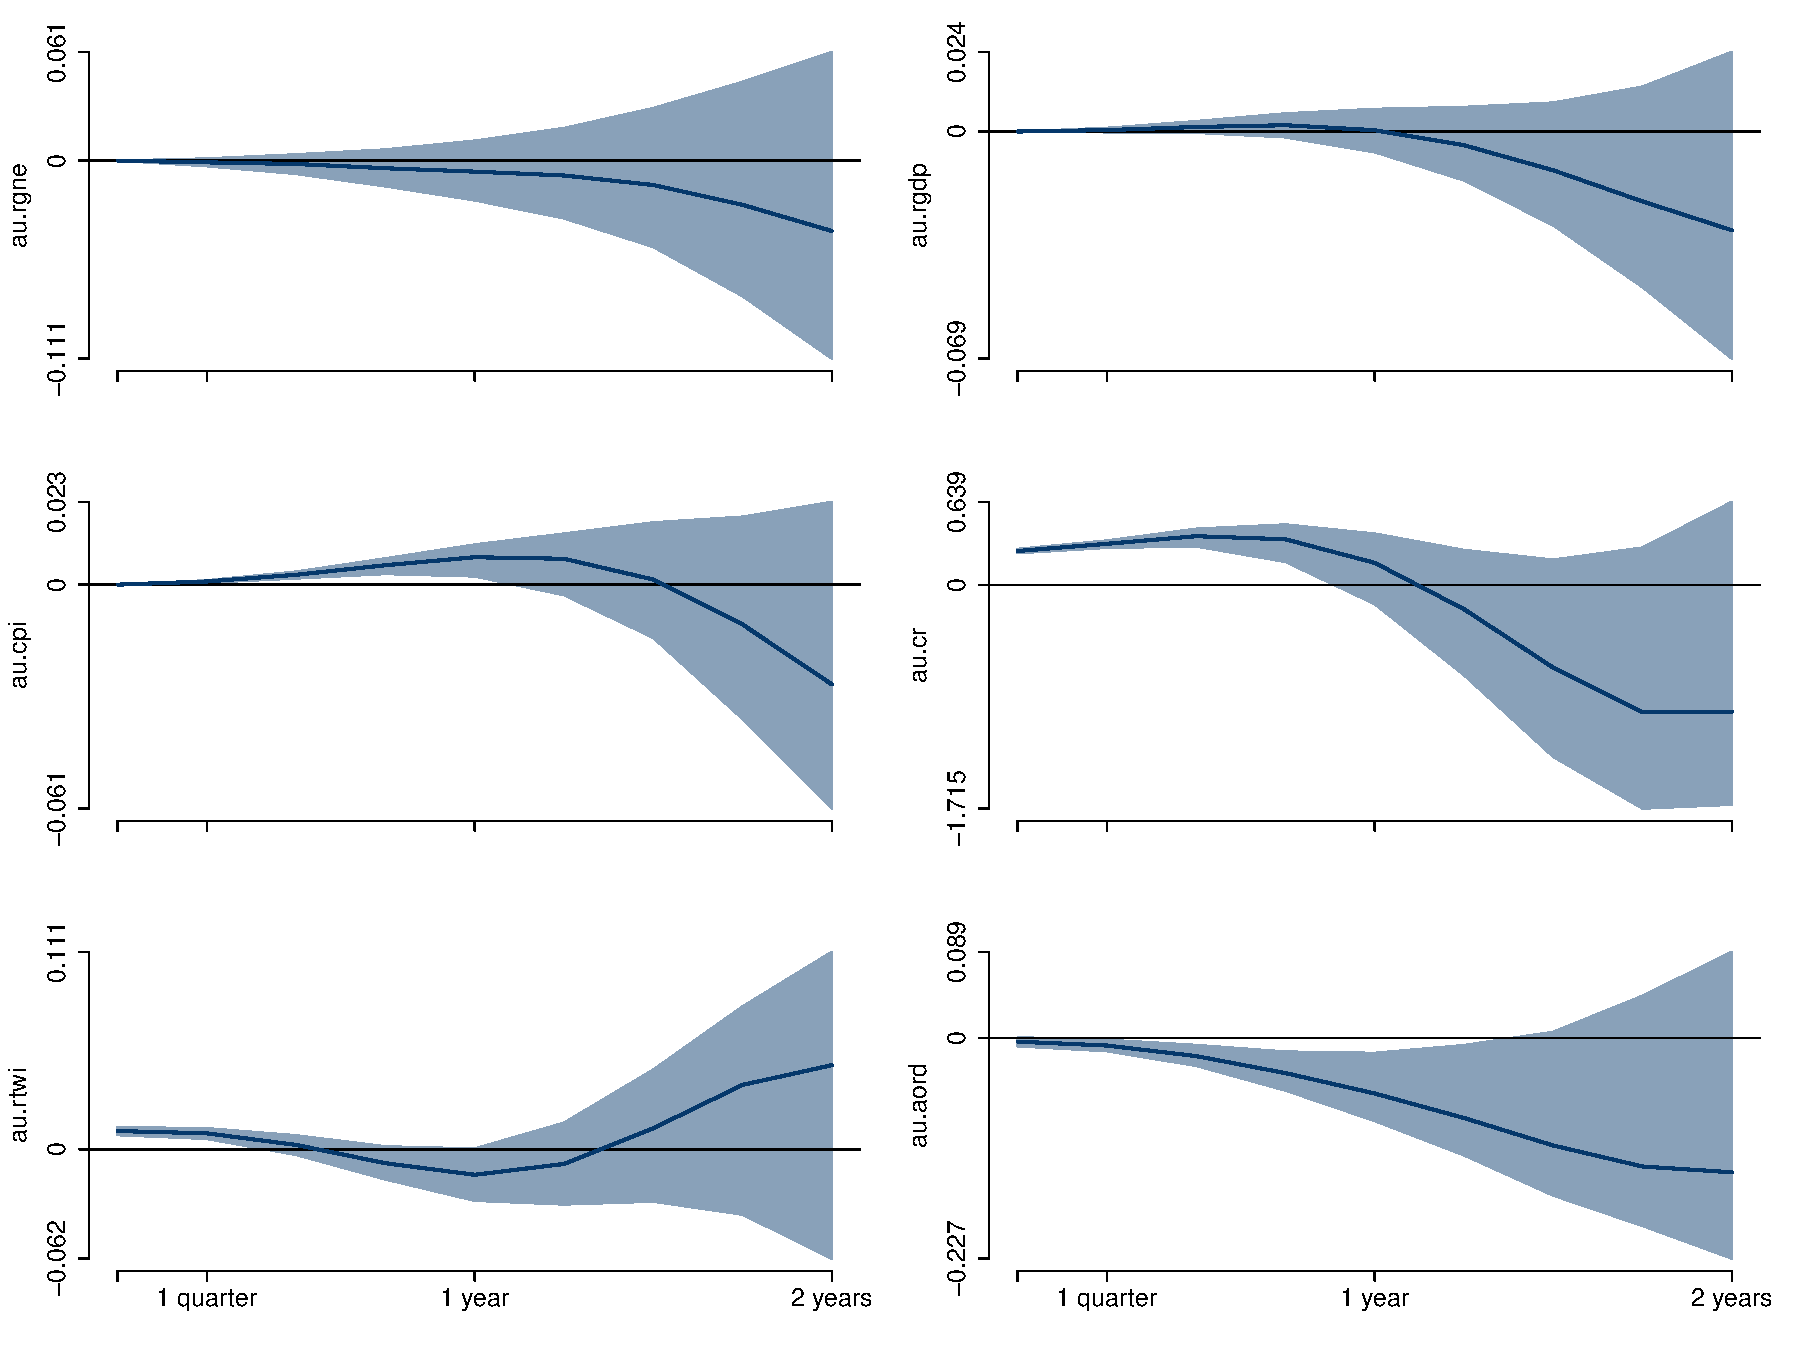
\includegraphics[scale=0.35]{irf-au-mps.pdf}

\end{frame}



\begin{frame}{IRFs to $u_{10.t}^{au.mps}$ for {\color{mcxs1}$\kappa_1=1$} and {\color{mcxs2}$\kappa_1=0.02^2$}}

\centering
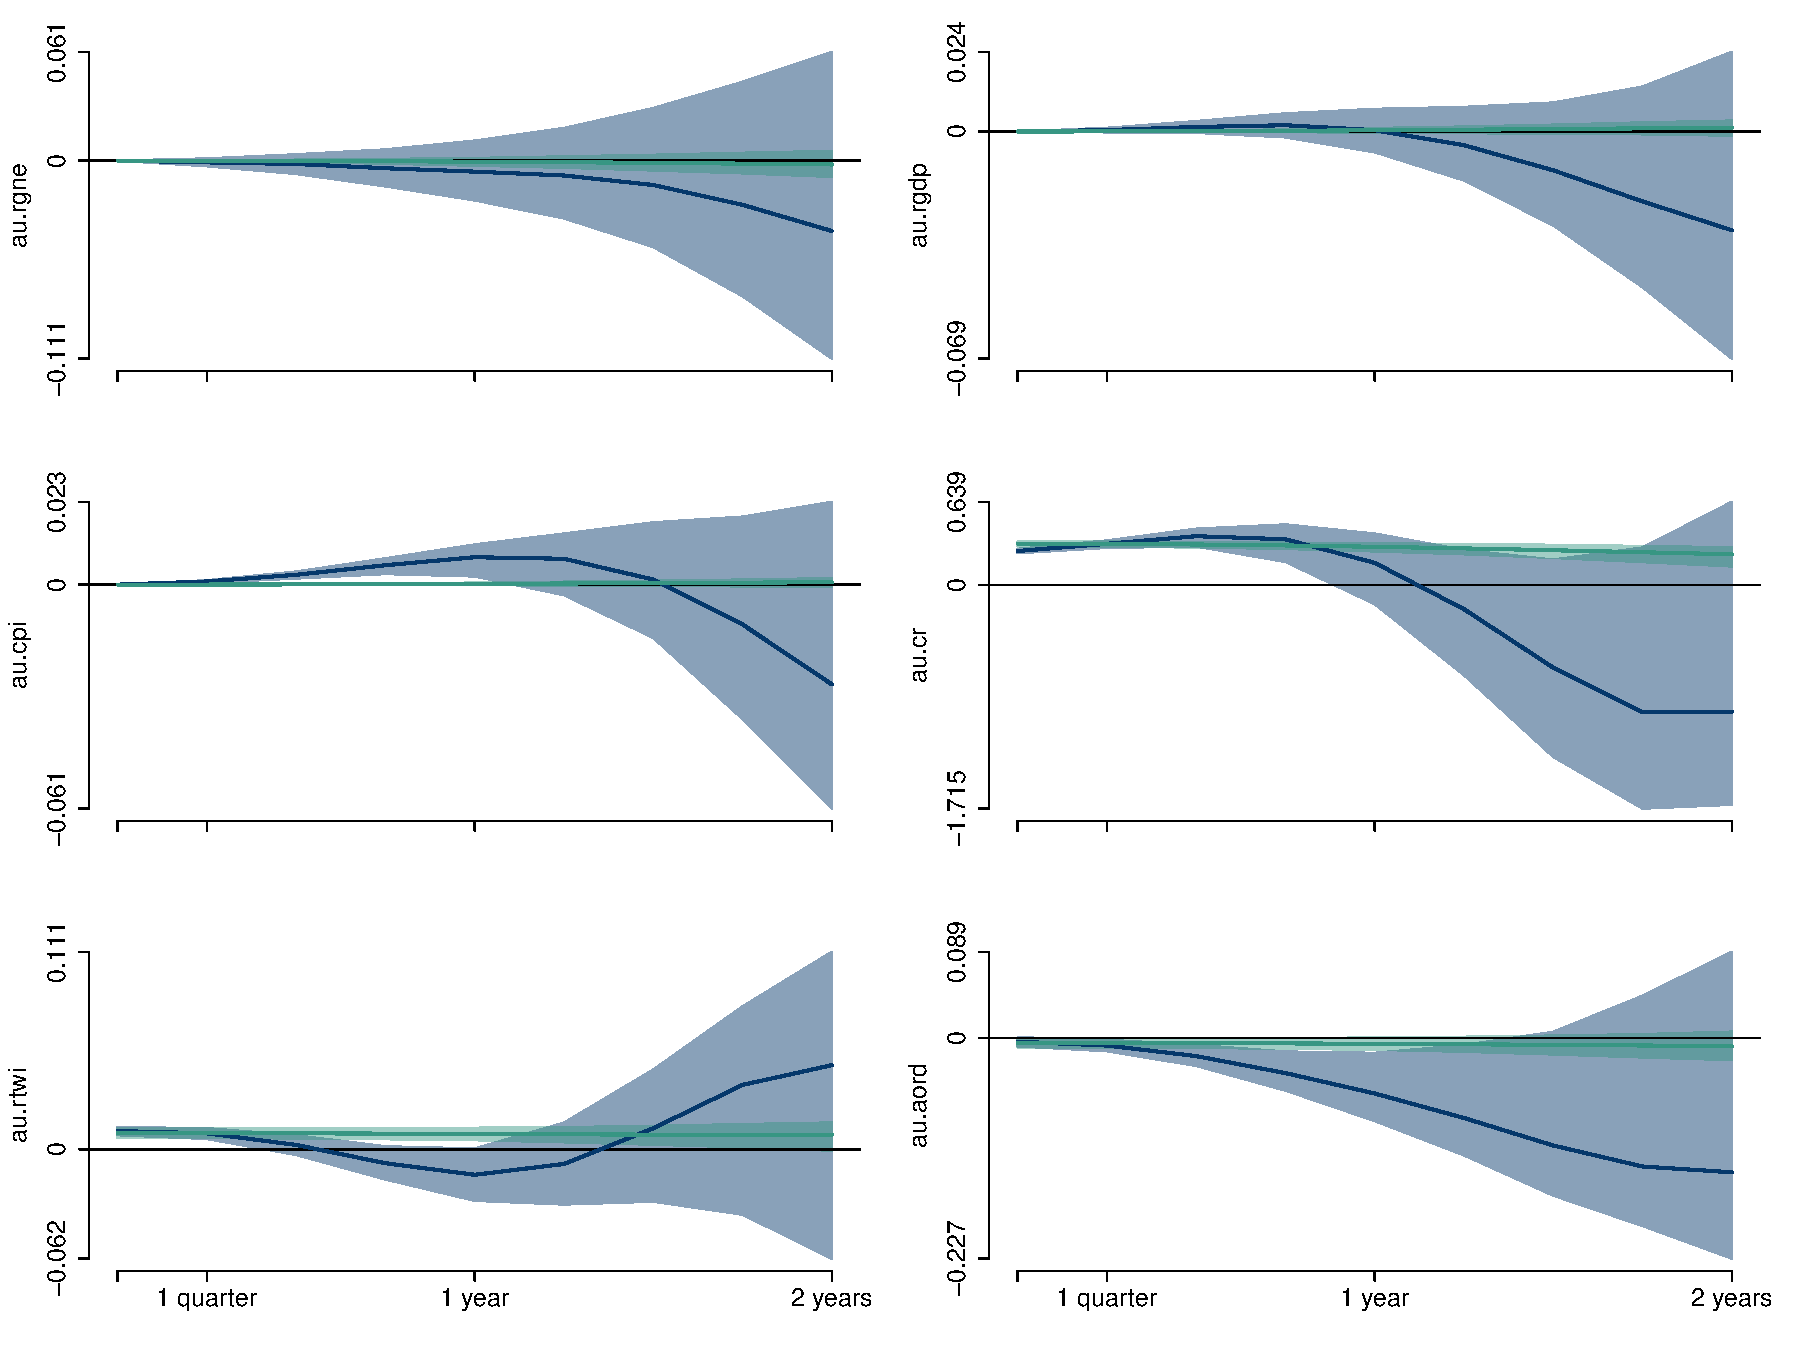
\includegraphics[scale=0.35]{irf-au-mps-both.pdf}

\end{frame}





{\setbeamercolor{background canvas}{bg=mcxs4}
\begin{frame}

\begin{adjustwidth}{-0.5cm}{0cm}
\vspace{8.3cm}\Large
\textbf{{\color{mcxs2}Forecast error variance} {\color{mcxs1}decomposition}}
\end{adjustwidth}

\end{frame}
}





\begin{frame}{Forecast error variance decomposition}

\textbf{Definition.}

\smallskip{\color{mcxs2}Forecast error variance decomposition provides information regarding the fraction of variability of the} $h${\color{mcxs2}-period ahead forecast of a particular variable attributed by each individual structural shock occurring at time} $t$.

\end{frame}




\begin{frame}{Forecast error variance decomposition}

\textbf{Forecast error variance.}\small
\begin{align*}
\mathbb{V}\text{ar}[\mathbf{e}_{t+h|t}] &= \mathbb{E}[(y_{t+h}-y_{t+h|t})(y_{t+h}-y_{t+h|t})'] \\
&= \mathbb{E}[\mathbf{e}_{t+h|t}\mathbf{e}_{t+h|t}'] \\
&= \mathbb{E}[(\Phi_0\epsilon_{t+h} +\dots + \Phi_{h-1}\epsilon_{t+1})(\Phi_0\epsilon_{t+h} +\dots + \Phi_{h-1}\epsilon_{t+1})'] \\
&= \mathbb{E}[(\Theta_0u_{t+h} +\dots + \Theta_{h-1}u_{t+1})(\Theta_0u_{t+h} +\dots + \Theta_{h-1}u_{t+1})'] \\
&= \Theta_0\mathbb{E}\left[\mathbb{E}_{t+1}[u_{t+h}u_{t+h}']\right]\Theta_0' + \dots + \Theta_{h-1}\mathbb{E}\left[\mathbb{E}_t[u_{t+1}u_{t+1}']\right]\Theta_0' \\
&= \Theta_0\Theta_0' + \dots + \Theta_{h-1}\Theta_{h-1}'\\
\end{align*} 
{\color{mcxs2}Focus on the diagonal elements of the matrix above.}
\end{frame}






\begin{frame}{Forecast error variance decomposition}

\textbf{Individual shock contribution.}

{\color{mcxs2}The contribution of the} $i${\color{mcxs2}th shock to the mean square forecast error (MSFE) of the} $n${\color{mcxs2}th variable} $y_{n.t+h}$ $h$ {\color{mcxs2}periods ahead is}
$$ \frac{MSFE_i^n(h)}{\sum_{j=1}^{N}MSFE_j^n(h)} $$

\bigskip where
$$ MSFE_i^n(h) = \theta_{ni.0}^2 + \dots + \theta_{ni.h-1}^2 $$
{\color{mcxs2}such that}
$$ \frac{MSFE_1^n(h)}{\sum_{j=1}^{N}MSFE_j^n(h)} + \dots + \frac{MSFE_N^n(h)}{\sum_{j=1}^{N}MSFE_j^n(h)} = 1$$

\end{frame}





\begin{frame}{Forecast error variance decomposition of $au.rgdp_{t+h|t}$}

\centering
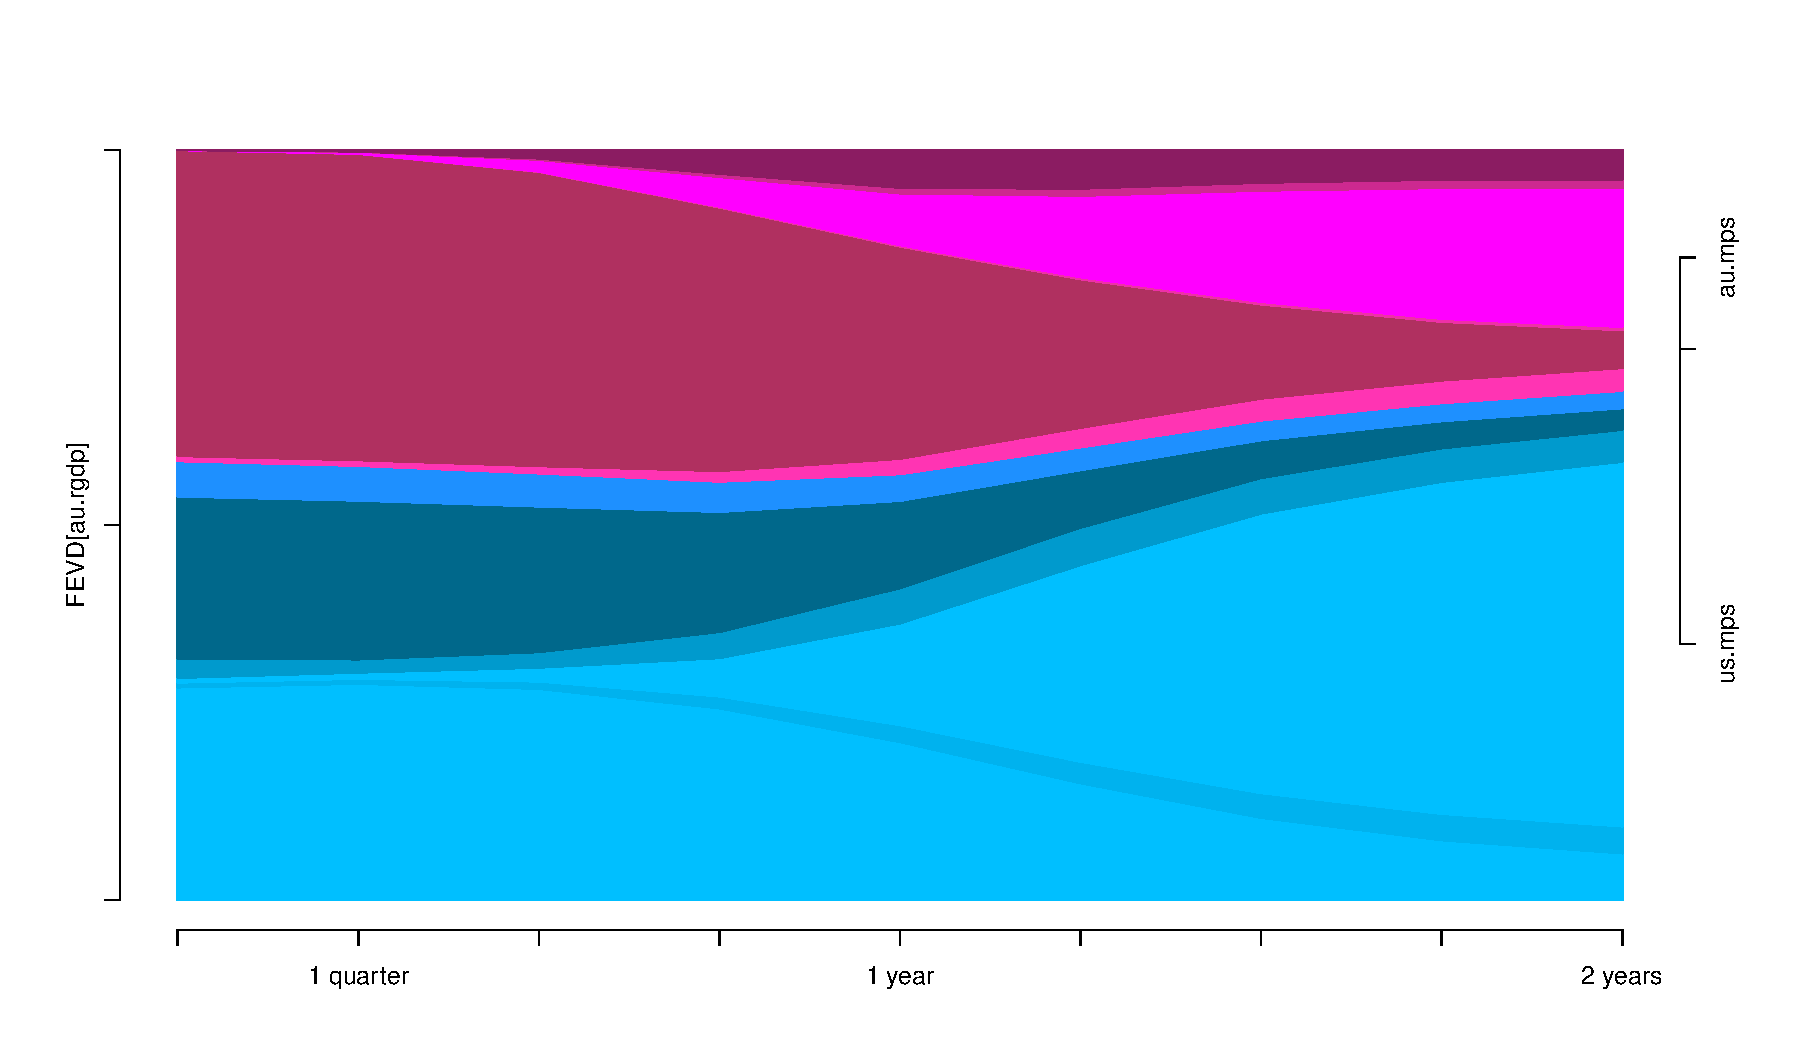
\includegraphics[scale=0.37]{fevd-au-gdp-k1.pdf}

\small{\color{mcxs2}Results for $\kappa_1=1$}
\end{frame}









\begin{frame}{Forecast error variance decomposition of $au.cpi_{t+h|t}$}

\centering
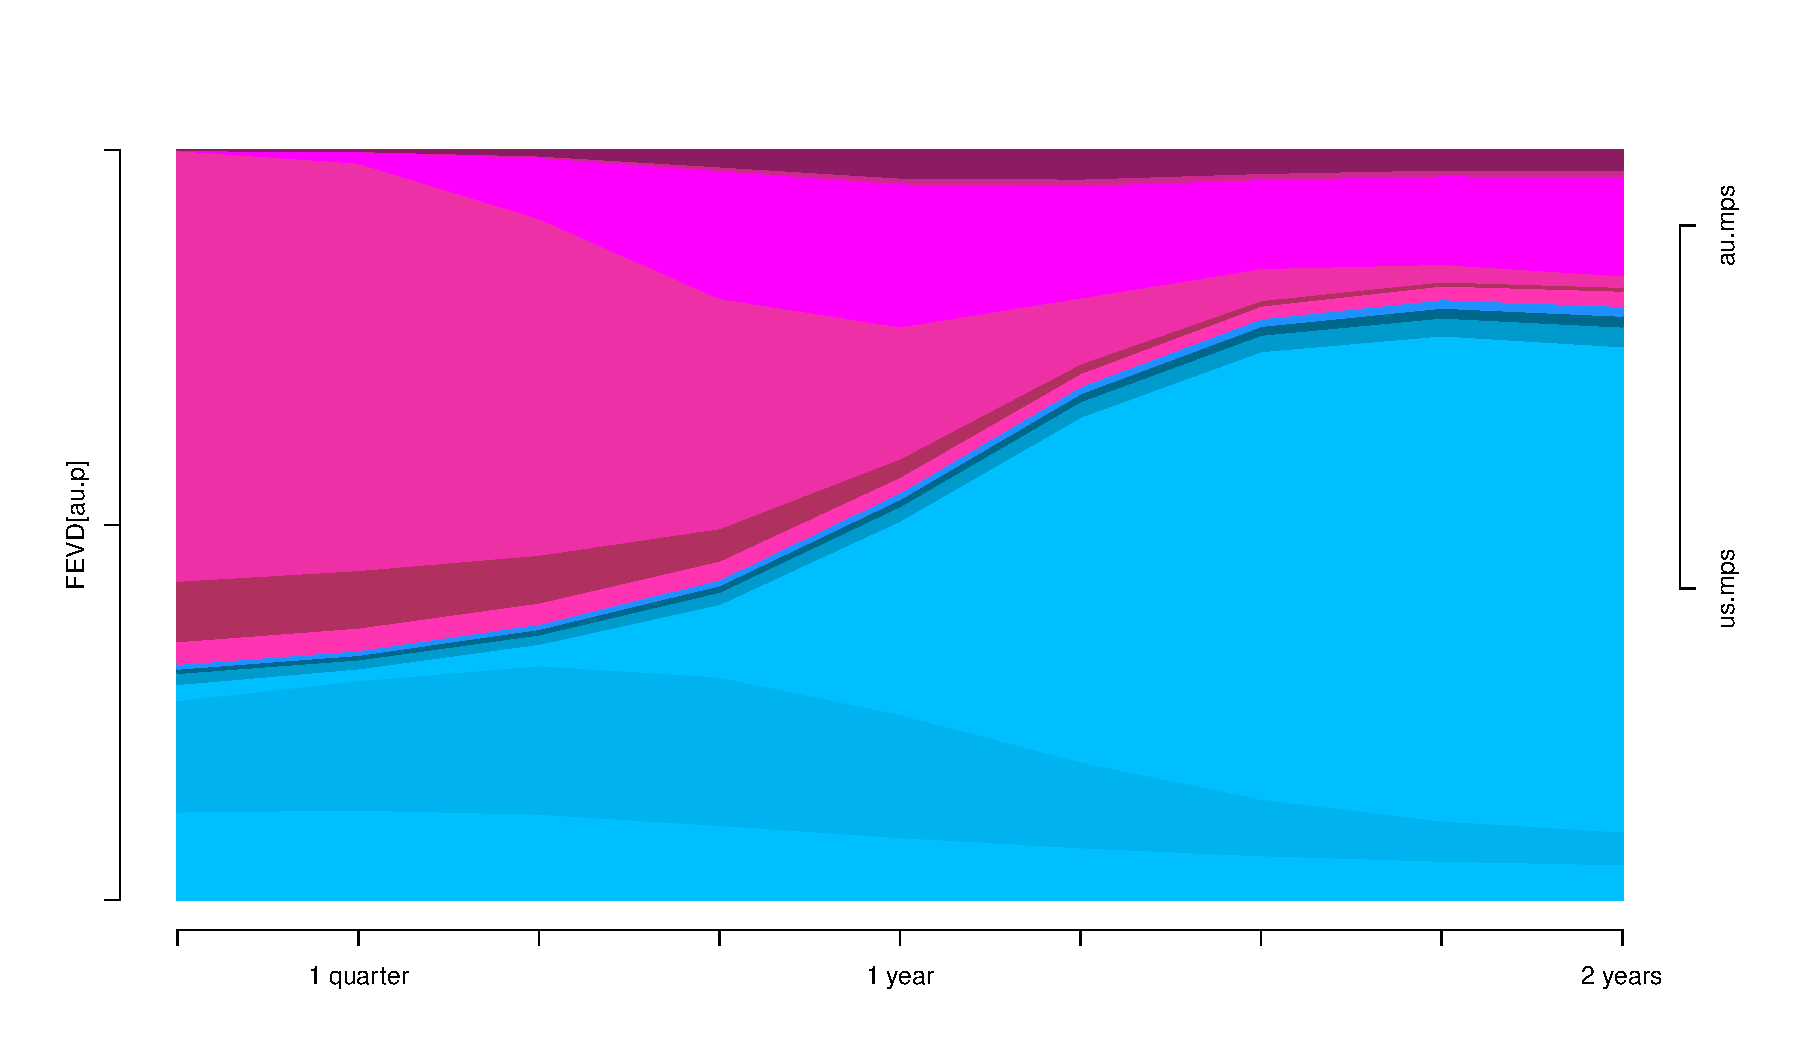
\includegraphics[scale=0.37]{fevd-au-p-k1.pdf}

\small{\color{mcxs2}Results for $\kappa_1=1$}
\end{frame}







\begin{frame}{Forecast error variance decomposition of $au.rgdp_{t+h|t}$}

\centering
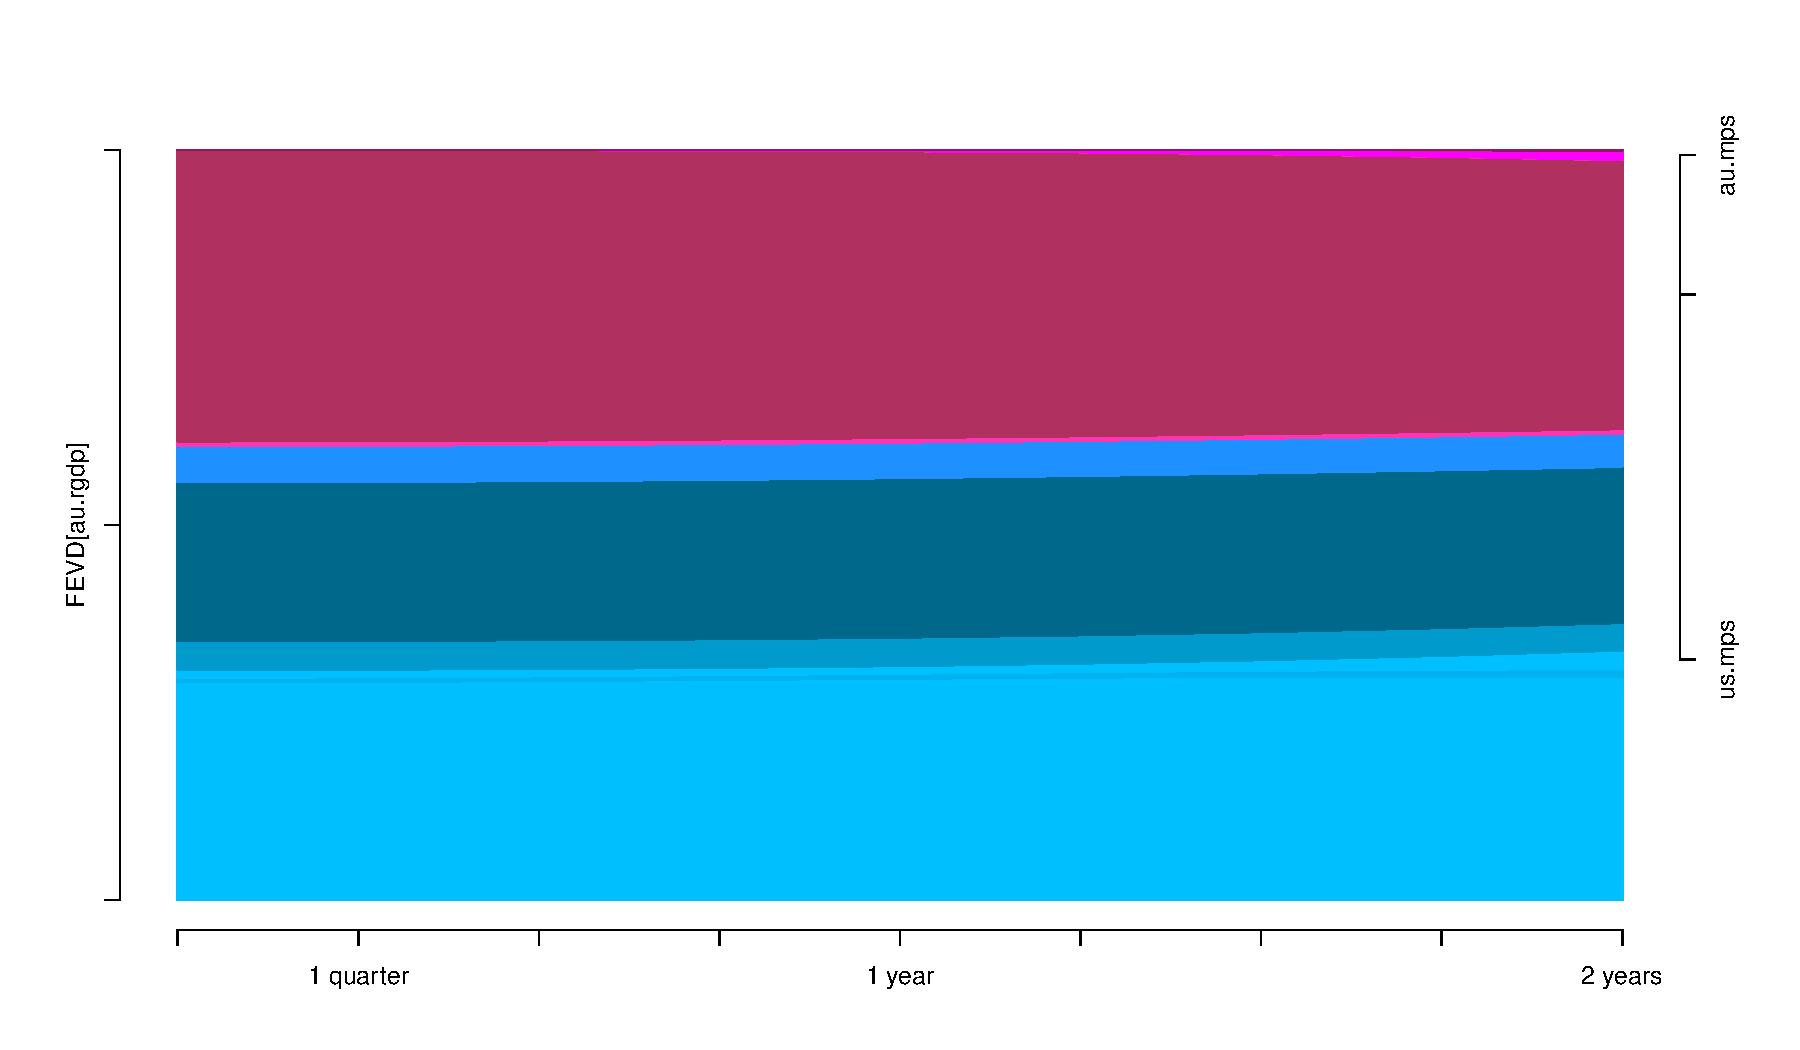
\includegraphics[scale=0.37]{fevd-au-gdp-k002.pdf}

\small{\color{mcxs2}Results for $\kappa_1=0.02^2$}
\end{frame}




\begin{frame}{Forecast error variance decomposition of $au.cpi_{t+h|t}$}

\centering
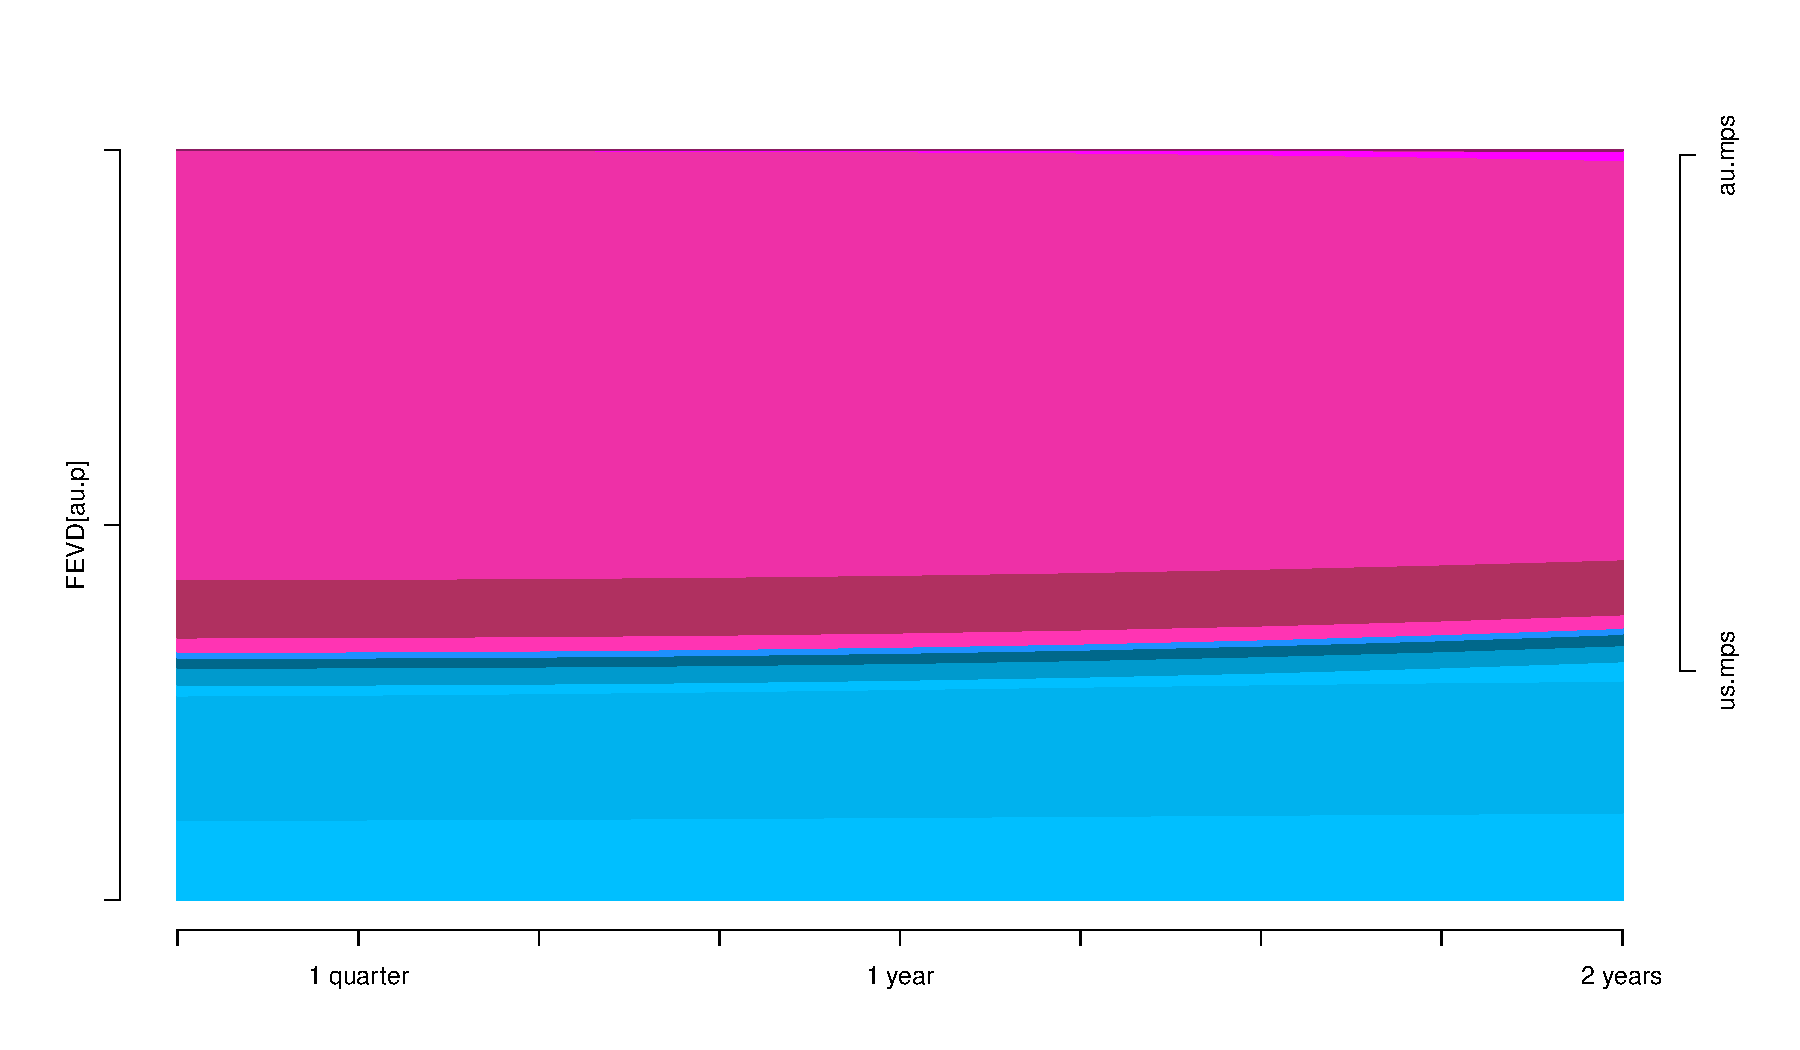
\includegraphics[scale=0.37]{fevd-au-p-k002.pdf}

\small{\color{mcxs2}Results for $\kappa_1=0.02^2$}
\end{frame}









%{\setbeamercolor{background canvas}{bg=purple}
%\begin{frame}
%
%\begin{adjustwidth}{-0.5cm}{0cm}
%\vspace{8.3cm}\Large
%\textbf{{\color{lightgray}Historical} {\color{white}decomposition}}
%\end{adjustwidth}
%
%\end{frame}
%}




%\begin{frame}{Historical decomposition}
%
%\textbf{Definition.}
%
%\smallskip{\color{mcxs2}The historical decomposition calculates the cumulative contribution of each shock to the observed unexpected change in the variables between two periods.}
%
%\begin{align*}
%y_{t+h} &= \Theta_0u_{t+h} + \Theta_1u_{t+h-1} + \dots + \Theta_{h-1}u_{t+1} + y_t\\
%y_{t+h}-y_t &= \Theta_0u_{t+h} + \Theta_1u_{t+h-1} + \dots + \Theta_{h-1}u_{t+1}
%\end{align*}
%
%{\color{mcxs2}The contribution of the} $i${\color{mcxs2}th shock to the observed unexpected change in the} $n${\color{mcxs2}th variable between periods} $t$ {\color{mcxs2}and} $t+h$ {\color{mcxs2}is equal to}
%$$ \mathbf{H}^n_{i}(h) = \sum_{l=0}^{h} e_{n.N}'\Theta_l e_{i.N} e_{i.N}'u_{t+h-l}$$
%
%{\color{mcxs2}where} $e_{i.N}$ {\color{mcxs2}is the} $i${\color{mcxs2}th column of} $I_N$
%\end{frame}





{\setbeamercolor{background canvas}{bg=mcxs4}
\begin{frame}{SVAR Tools}
\begin{description}
\item[Estimation output] {\color{mcxs2}for structural models can be used to compute a wide range of economically interpretable values.}

\bigskip\item[Structural shocks] {\color{mcxs2}that have statistically significant IRFs over some period and contribute to a large extent to the FEVDs are considered the main drivers for economic measurements}

\bigskip\item[The monetary policy shock] {\color{mcxs2}can be considered a non-negligible determinant of the business cycle in Australia}
\end{description}
\end{frame}
}

\end{document} 